\chapter{使用した技術}
%rosについてもっと深堀する
%例:パッケージの作り方,ノードの作り方,パブリッシャーとはなにか,サブスクライバーとはなにか
%ROSのパブリッシャーとサブスクライバーの作り方,mROS 2の作り方embeddedRTPSについても話せるとよい
%C++とpythonの違いを述べる.本実装ではなぜC++を選択したのかを書く
%ついでにサービスとアクションについても述べる
%messageの中身についても語りたい.後で説明が楽になる
\label{sec:usage}
\section{ROS 2}
 ROS 2は,ROSの後継であり,ROS 2はROS 1と比べて,分散型のロボットシステムに対応している.
ROS 1では,主にUDPを使用したメッセージ型の通信を行っていたが,ROS 2では,DDS(Data Distribution Service)[?]と呼ばれる通信ミドルウェアを採用しており,RTPS(Real Time Publish Subscribe)プロトコルを用いた
メッセージ型通信を行っている.これによって,個々のロボットが独立して動作するだけでなく,複数のロボットが協調して動作することが可能になった.
現在はROS 2が主流であるが,ROSは,スタンフォード人工知能研究所の研究プロジェクトとから移管されたWillow Garage社によって開発が始まっているロボットソフトウェア開発基盤である.
最初の正式なディストリビューション版は,2010年3月にリリースされたBox Turtleである.
ROSの利点は,分散型ロボットシステムの実現に向いている通信ミドルウェア,プロジェクト管理やデバックおよびシュミレーションなどのためのツール群,
再現性の高い豊富なOSSのパッケージやライブラリ,世界規模の活発なオープンソース開発コミュニティという4つの側面にある[?].
すでに10年以上の歴史を持っており,ロボット工学の発展にROSは大きく貢献してきた.日本の企業ではソニーのaiboの事例がROSを使った製品として代表的であり,企業でも商用商品に採用されることも多い.
ロボット開発を開発を取り巻く環境やROSが研究用から商用にも活用され始めるという変遷を受け,2014年より第2世代バージョンであるROS 2の開発が始まった.
ROS 1の思想を踏襲しながらも,その基本設計から見直し,一から実装しなおされている.2015年8月には最初のdistributionであるArdent Apaloneがリリースされた.
現在はubuntu22.04やwindows,macOSなどにも対応したROS 2 humbleディストリビューションがリリースされている.

\subsection{パブリッシャーとサブスクライバー}
 ROSでは基本的なノード間のデータ通信としてパブリッシューサブスクライブ通信型の非同期な通信方式がある.データの送信側をパブリッシャー(Publisher,出版者)とよび,受信側をサブスクライバー(Subscriber,購読者)という.
通信経路として,定義であるトピック(Topic)を介した通信が行われる.トピックで送受信されるデータはメッセージ(Message)と呼ばれ,車輪の角速度や回転量や現在位置の3次元座標など,基本型を組合せた任意の型を定義することができる.
同じ名前のトピックに対して,様々な個数や種類のノードが任意のタイミングで登録や変更,削除ができる.
さらに,メッセージの型が一致していれば,メッセージの通信が行われる.
パブリッシュ側は自由なタイミングで動作でき,非同期に動作するサブスクライバー側は,パブリッシュ側では対応するコールバック関数が実行される.
ノードはパブリッシャーにもサブスクライバーにもプログラム次第で変化できるため,ユーザがオリジナルのノードを作成することができるため,ノード同士の依存が少なくなり,ロボットシステム全体の機能の追加や削除が容易であるため,柔軟なロボットシステムを構築できる.
また,ROS 2ではパブリッシャーはrclcpp::Publisherクラスを,サブスクライバーはrclcpp::Subscriptionクラスを使用して実装する.
\\ ROS 2の通信ミドルウェアであるDDSと通信プロトコルであるRTPSは,通信相手の探索および通信経路の確立を自律的に行う.
この機能の実現は,RTPSのSPDP(Simple Participant Discover Protocol)というプロトコルによって行われる.およびSEDP(Simple Endpoint Discover Protocol)が備えられている.ここで,RTPSでは,ROS 2のノードに相当するものをParticipant(参加者)と呼ぶ.
通信相手を探索するためには自身の情報を送信するモジュールをWriter,ほかのParticipantから情報を受け取るモジュールをReaderと呼ぶ.
SPDPは,Participantの情報を送受信するためのプロトコルであり,SEDPは,Topicの情報を送受信するためのプロトコルである.
この通信のエンドポイントは,Participant同士のパブリッシュ,サブスクライブである.
\\ RTPSをOSI参照モデルに例えるとtransport層に位置し,UDP/IPの上に実装されている.UDP通信にはパケットの到着に関する保証がないが,ROS 2のDDSではこれを補助するQoS(Quality of Service)制御の機能がある.
QoS制御は,サブスクライバ,パブリッシャごとに設定でき,厳格な条件であればRELIABLE(信頼性の高い通信)を,緩やかな条件であればBEST EFFORT(ベストエフォート通信)を選択することができる.
ROS 2のデフォルトDDSであるFastRTPSでは,QoS制御の機能が実装されており,各ノードが通信するときのQoS設定はRELIABLEである.
\subsection{ノードの作り方とパッケージ}
 ROS 2においてノードを作成する場所は決まっており,一般的にはros2\_ワーキングスペース(ws)というディレクトリを作った後,その中にsrcというディレクトリを作成し,その中にノードを作成する.
srcディレクトリを作成した後,ros2\_wsディレクトリでcolcon buildというコマンドを実行することで,ros2\_wsの中でノードを作成することがきる.
ROS 2の場合,ノードの集まりのことをパッケージと呼ぶ.
パッケージはros2 pkg createというコマンドを実行することで作成することができ,srcディレクトリの直下で実行することで,パッケージを作成することができる.
パッケージを作成する前にそのパッケージの中で使用する言語を決める必要がある.
ROS 2はC++とPythonの2つの言語をサポートしており,ユーザーの好みに合わせて変更できる.
\subsection{オーバーレイとアンダーレイ}
また,ROS 2には重要な概念にアンダーレイとオーバーレイがある.
アンダーレイは,完成されたパッケージをインストールするワークスペースであり,安定した環境をオーバーレイに提供するためにある.
オーバーレイは,ユーザー自身で作成したパッケージを扱うワークスペースであり,先ほどのros2\_wsはオーバーレイにあたる.
ROS 2ではユーザーが作るノードやパッケージをオーバーレイに作成し,必要に応じてアンダーレイのパッケージを参照して使用するのが一般的である.
このオーバーレイ上でユーザはcolcon buildを実行し,パッケージをビルドする.
ユーザーはパッケージをビルドした後,すぐに実行することができない.ROS 2ではsourceコマンドを用いてオーバーレイ環境を読み込むことでアンダーレイがオーバーレイより優先されることなく,開発することができる.
ROS 2においてオーバーレイとアンダーレイは,複雑化するロボットシステムに柔軟性と拡張性をもたらす概念であることがわかる.
ROS 2のデバック方法として様々なコマンドが用意されており,ros2 topic listというコマンドを実行することで,現在実行されているトピックの一覧を表示することができる.
また,現在実行されているノードを視覚的に確認できるようにrqt\_graphと呼ばれるものが用意されている.開発者はrqt\_graphを用いて,目に見えないROS 2のノード間の通信を確認することができる.
こうしたアンダーレイ機能の充実によって,ROS 2はROS 1よりも柔軟性と拡張性を持つことができた.
\subsection{ROS 2が対応しているDDS}
ROS 2にはデフォルトでFastRTPSというDDSが実装されている.
DDSとは,OMG(Object Management Group)が定めたデータ交換のための仕様である.これによって分散型ネットワークでも効率的に通信が可能になっている.
FastRTPSのほかにも,RTI Connext DDSやeProsima Micro XRCE-DDSというDDSがROS 2に対応している.
Ubuntu22.04のROS 2 humbleでは,FastRTPSはもちろんのこと,デフォルトでEcripse Cyclone DDS,Gurum DDS,RTI Connext DDSがインストールできる.%リファレンス1[https://docs.ros.org/en/humble/Installation/DDS-Implementations.html#ubuntu-linux-source-install].
\subsection{サービスとアクション}
ROS 2では,パブリッシャーとサブスクライバー以外にもサービス通信とアクション通信がある.
サービス通信は,サーバーとクライアントの2つのノード間でリクエストとレスポンスをやり取りする通信である.
これは既存のクライアントーサーバーモデルによく似ており,Subscribeするのではなく,ノードがメッセージの値を欲しいタイミングでリクエストする仕組みになっている.
そのため,ロボットに対する命令やデータの取得,計算結果を受け渡しに適しており,サービス通信はリアルタイム性や連続的なデータには向かないが,確実に応答するというロボットシステムにおいて重要な役割を果たす.
さらに,サービス通信は同期的な通信であるため,サービス通信を行うノードは,サービス通信が完了するまで他の処理を行うことができない.
そのため,クライアントの処理を間接的にブロックすることができる.
一方,アクション通信は,サービス通信と同様にサーバーとクライアントの2つのノード間でリクエストとレスポンスをやり取りする通信である.
しかし,アクション通信はサービス通信と異なり,リクエストに対するレスポンスを即座に返すのではなく,リクエストに対するレスポンスを返すまでの間に,進捗状況を返すことができる.
この通信方式によって,長時間のタスクやフィードバックが可能なタスク,中断可能なタスクに適しているため,開発者は柔軟性を保ちながら,ロボットシステムを構築することができる.
さらに,アクション通信は非同期的な通信であるため,アクション通信を行うノードは,アクション通信が完了するまで他の処理を行うことができる.
これによって,複雑なタスクを行うノードでもアクション通信を用いることで同時に処理することが可能であり,多くのリソースがあるマシンで高度なノードを動作させることができる.
実装方式として,サービス通信は,ROS 2ではrclcpp::Service,Clientクラスを用いて実装する.アクション通信は,ROS 2ではrclcpp::ActionServer,Clientクラスを用いて実装する.
%サービス通信は,ROS 2ではrclcpp::Service,Clientクラスを用いて実装する.

\section{mROS 2-POSIX}
\begin{figure}[ht]
    \centering
    \begin{minipage}{.48\textwidth}
        \centering
        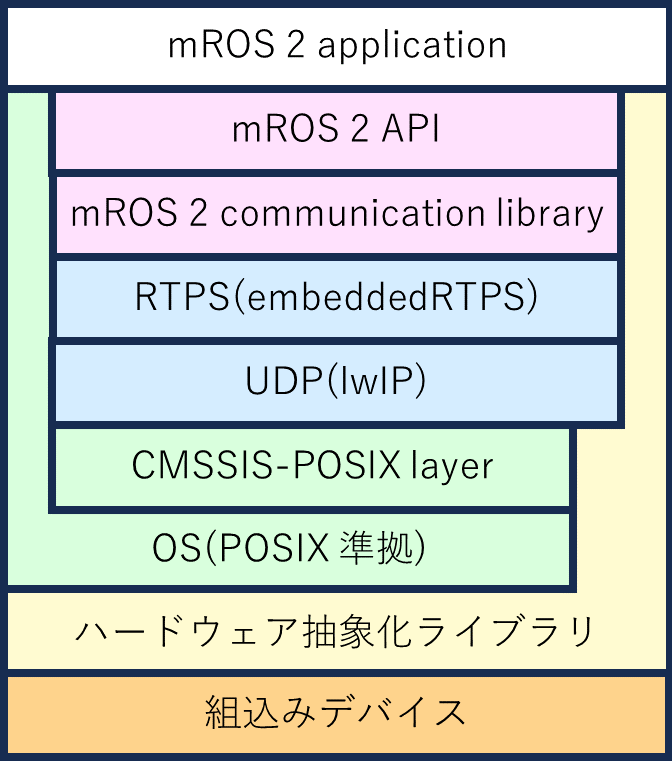
\includegraphics[width=0.9\linewidth]{images/fig1_mros2posix_a.png}
        \caption{mROS 2-POSIXの内部構成}
        \label{fig:subfig_a}
    \end{minipage}
    \hfill
    \begin{minipage}{.48\textwidth}
        \centering
        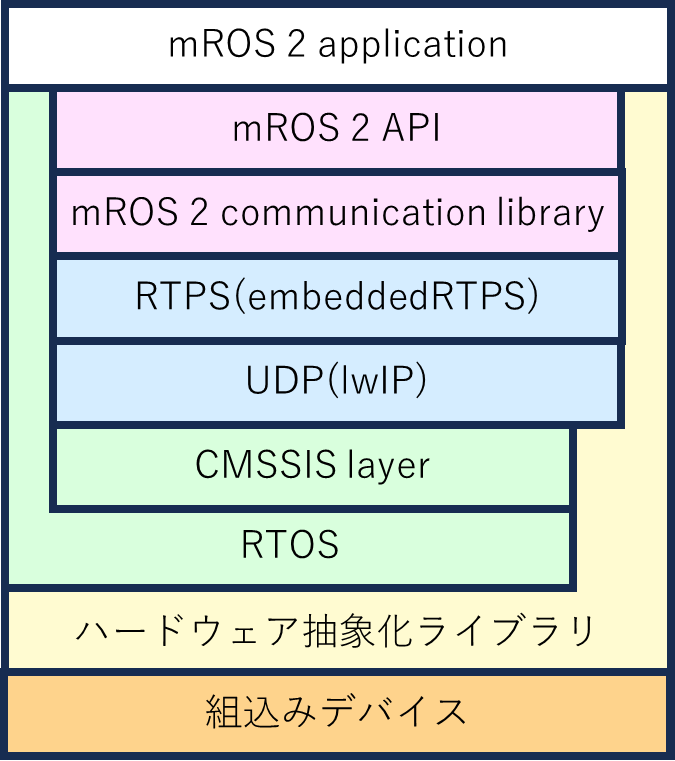
\includegraphics[width=0.9\linewidth]{images/fig1_mros2_b.png}
        \caption{mROS 2の内部構成}
        \label{fig:subfig_b}
    \end{minipage}
\end{figure}
\subsection{mROS 2}
mROS 2は,ROS 2ノードの軽量実行環境である.
ROS 2を採用するロボットシステムにおいて通信方式とメモリ軽量な実行環境を確立することができる組み込み技術を導入することにより,分散型のロボットシステムにおける応答性やリアルタイム性の向上,消費電力の削減が可能になる.
mROS 2は汎用OS上で実行されるROS 2ノードと通信できることを目的として実装された.
そのため,パブリッシューサブスクライブ通信の相手と経路を自律的に探索できるように設計され,ROS 2およびRTPSの利点が,組み込み技術導入時に損なわれないようになっている.
ROS 2に対応しているDDSの種類として,FastRTPS,RTI Connext DDS,eProsima Micro XRCE-DDSを挙げたが,既存の組込みデバイス向けのROS 2ノード実行環境であるmicro-ROS[?]がある.
micro-ROSはRTPSの軽量規格であるDDS-XRCE(DDS For Extremely Resource Constrained Enviroments)[?]の実装であるMicro XRCE-DDS[8]を採用している.
Micro XRCE-DDSは,ホストとしてROS 2ノードを実行するデバイスと通信する際に,Agentノードと呼ばれるノードの稼働が必要となる.
通信の仲介の役割をAgentノードはになっており,Agentノードは,ホストデバイス上のROS 2ノードとRTPSに則った通信,組み込みデバイス上のノードとXRCEに則った通信がそれぞれ行われるため,
応答性とリアルタイム性の低下が懸念される.また,複数の組み込みデバイスを用いる場合,Agent ノードは分散型システム全体の通信を仲介するため,Agentノードの数が増えると通信の遅延が増加する.
そのためmROS 2は,DDSとしてXRCE-DDSを採用せず,embeddeRTPS[?]を採用している.
embeddeRTPSは,一つのDomainクラスからParticipant,Writer,Readerの3つのインスタンスが生成される.つまり,初期化処理の段階でembeddedRTPSの提供するパブリッシューサブスクライブ通信が利用できるようになる.
これによってXRCE-DDSのようにAgentノードが必要なく,組み込みデバイス上での通信の遅延を抑えることができる.
このembeddeRTPSが採用されたのは通信の遅延を抑えることができるだけではない.
このRTPSは,SPDPとSEDPが実装されており,通信の宛先や受け手として自立性を確保できるRTPSであること点である.
また,ROS 2で代表的なFastRTPSと通信の確認ができているため親和性が高い点も上げられる.
以上の設計思想によりmROS 2は,計算資源の限定的な組み込みデバイス上での稼働を想定した組込みデバイスのリアルタイム性の向上および消費電力の削減ができるソフトウェア基盤である.
\subsection{mros2の内部構成}
図1(a)にmros2の内部構成を示す.
ユーザーアプリケーションからの階層順で,mROS 2通信ライブラリ,通信プロトコルスタック,RTOS,ハードウェア抽象化ライブラリによって構成される.
mROS 2通信ライブラリは,ユーザアプリケーションに対して,ROS 2通信のトピックに関する基本的なAPIを提供している.
主なAPIとして void mros2::init(),void mros2::Node::create\_node(),void mros2::Publisher::create\_publisher(),void mros2::Subscriber::create\_subscriber()がある.
通信プロトコルスタックには,C++で実装されたembeddedRTPSを採用している.先ほど述べたようにこのRTPSにはSPDPとSEDPが実装されており,計算資源の限定的な組込みデバイス上での稼働を想定した設計であるかつ,ROS 2の代表的なRTPSであるFastRTPSと通信の確認できているという理由がある.
UDPについては組込み向けのCによる軽量実装であるlwIP[?]が採用されている.
RTOSには,TOPPERS/ASP3カーネル[?]が採用されており,高分解能大麻やティックレスの低消費電力な処理遅延機能など,高いリアルタイム性と安全性が求められる軽量な組込みシステムに適した設計がなされている.
lwipはCMSIS-RTOS APIに依存しているため,それぞれのAPI差分を吸収するラッパが用意されている.
\subsection{mROS 2の通信機能}
mROS 2の通信機能は,mROS 2の通信ライブラリにあるinit task(初期化処理)とRTPS/UDPと通信ライブラリを介するwrite task(パブリッシュ処理)とreader task(サブスクライブ処理)の3つのタスクに分けられる.
またアプリケーション層にあるuser task(ユーザーアプリケーション)という開発者が実装するタスクがある.
user taskは,ROS 2のノードに相当している.パブリッシューサブスクライブ通信を行うアプリケーションである.
mROS 2のAPIを介してパブリッシュやサブスクライブを行うことができる.
init taskはROS 2としてのノードの情報の初期化を行う.APImros2::init()が呼ばれたときに,対象の組込みデバイスをRTPSのParticipantとして登録する.
writer taskとreader taskに関しては,パブリッシュおよびサブスクライブに関する処理を担う.これらのタスクはuser taskからの依頼をmROS 2APIを介して受け,RTPSの該当機能を立ち上げる.
writer taskはパブリッシュの依頼を受けて起動し,reader taskはサブスクライブの依頼を受けて起動する.
\subsection{mROS 2-POSIXの内部構成}
そして,mROS 2がPOSIX[7]に対応したのがmROS 2-POSIXである.
\\ 図1(b)は,mROS 2-POSIXのソフトウェア構成を示す.mROS 2-POSIXアプリケーション層は,ユーザが実装するROS 2ノードに相当する.
つまり,ROS 2におけるオーバーレイに相当する層である.
mROS 2-POSIX API層および通信ライブラリ層は,メッセージを非同期にパブリッシュやサブスクライブするためのコミュニケーションチャネルであるROS 2のTopicに相当するAPIおよび通信機能を提供する階層である.
本階層は,ROS 2のネイティブなクライアント通信ライブラリであるrclcppと互換性を保つように設計されている.
mROS 2通信ライブラリでは,rclcppのうちpub/sub通信の基本的な機能のみ実装されている.
利用可能な機能は制限されているものの,組込み技術を導入するROS 2開発者は,汎用OS向けのプログラミングスタイルを踏襲しながらC++によってmROS 2のアプリケーションを実装できる.
そのためmROS 2-POSIXはサービス通信やアクション通信には対応していない.
\\ RTPSプロトコルスタックにはUDPでパブリッシャとサブスクライバC++実装のembeddedRTPS[8]が採用されている.
UDPについては組込み向けのC実装であるlwIPが採用されている.
通信層のembeddedRTPSおよびlwIPはCMSAIS-POSIXに依存しており,図1(b)に示すmROS 2のCMSIS-RTOSを互換した層になっている.
最下層にはハードウェアを抽象化したライブラリがある.
\\ mROS 2-POSIXは図2に示す実行方式を採用している.
リアルタイムOSでは,組込みマイコンを実行資源の管理対象として,タスク単位でアプリケーションが実行される.
POSIXにおいてはタスクに相当する概念はプロセスであり,そこから生成されるスレッドを実行単位として処理が進行している.
しかし,mROS 2-POSIXは実行単位であるノードにPOSIXのスレッドを対応づけ,組込みマイコンでの通信処理におけるイベント割込みについては,POSIX準拠OSにおけるブロッキングAPIの発行に相当させて処理している.
これらの方式によって,mROS 2-POSIXはPOSIX準拠OS上で仮想ROS 2ノードとして軽量環境下で実行することができる.
\subsection{mROS 2-POSIXの動作フロー}
mROS 2-POSIXの動作は以下のようになっている.
\begin{itemize}
    \item netif\_posix\_add(NETIF\_IPADDR, NETIF\_NETMASK)によって,lwIPのネットワークインターフェースを初期化する.
    \item osKernelStart()によって,RTOSのカーネルを起動する.
    \item mros2::init(0, NULL)によって,mROS 2-POSIXの初期化を行う.
    \item mros2::Node::create\_node(ノード名)によって,ノードを生成する.
\end{itemize}
mROS 2-POSIXは通常のmROS 2と同様にlwipを利用してUDP stackを実装している.
異なる点として,mROS 2‐POSIXはPOSIXレイヤが設けられていることが挙げられる.
このように明確なレイヤを設けたことによって,netif\_posix\_add(NETIF\_IPADDR, NETIF\_NETMASK)のような実装が追加されている.
引数に現在mros2-posixをビルドしているマシンのIPアドレスとサブネットマスクを設定することによって,lwIPのネットワークインターフェースを初期化する.
このNETIF\_IPADDRとNETIF\_NETMASKは,mROS 2-POSIXのヘッダファイルであるmros2\_posix\_netif.hに定義されている.
そのためビルド前にip aなどで自分のIPアドレスを確認し,そのIPアドレスとサブネットマスクを設定する必要がある.
この設定をを行わないと,ROS 2やほかのmROS 2ノードと通信できなくなり,ros2 topic listなどのデバックコマンドにも表示されない.
\\ 次に,osKernelStart()によって,RTOSのカーネルを起動する.その後,mros2::init(0, NULL)によって,mROS 2-POSIXのノードの初期化を行う.
mros2::init()はmROS 2-POSIXのノードの初期化,つまり,ROS 2としてノード情報を初期化するということである.これは対象の組込みデバイスをRTPSのParticipantとして登録する.
このタスクを行った後,mros2::init()は休止状態に移行する.
\\ そして,mros2::Node::create\_node(ノード名)によって,ノードを生成する.この命令に紐づけられたインスタンス変数を介して,パブリッシャーやサブスクライバーを生成する.

\subsection{mROS 2-POSIXのパブリッシュ処理}
mROS 2-POSIXにおいてパブリッシュ処理はmROS 2とほとんど変更がない.
まず,mros2::Node::create\_publisher()によってmROS 2ノードをパブリッシャーとして登録する.
mros2::Node::create\_publisherは関数テンプレートとして実装されており,第一引数にトピック名,第二引数にパブリッシュするメッセージのキューのサイズを設定する.
例として,mros2::Node::create\_publisher<型>(トピック名,10)という形で記述する.
<型>の中に入るのは,パブリッシュするメッセージの型である.ROS 2同様に様々な種類の型を設定でき,ユーザーが自由に定義することができる.
同様に"トピック名"にはトピック名が,10はパブリッシュするメッセージのキューサイズ(履歴の長さ)が入る.
定義されたpublisherがどのようにパブリッシュされるのか以下にフローを示す.
\begin{itemize}
    \item mros2::Publisher.publish()を呼び出す.引数にはメッセージ情報が格納されたオブジェクトのポインタを渡す.
    \item mROS 2-POSIXの通信ライブラリ内でメッセージのシリアライズを行い,RTPSに則った形式に変換する.
    \item embeddedRTPSの提供する機能によってUDPパケットを作成し,タスク間通信でmROS 2-POSIXのParticipantのwriterにパブリッシュ処理を依頼する
    \item writerのタスクが実行され,RTPSのSPDPによって,パブリッシャー情報を送信する.
\end{itemize}
mROS 2‐POSIXのパブリッシュ処理は,mROS 2と同様にUDPパケットを作成し,RTPSのSPDPによって,パブリッシャー情報を送信する.
mROS 2通信ライブラリの通信処理効率化のためにwriter taskは,CPUとネットワーク通信を平行に行うことができる.
このため,embeddedRTPSやlwIPにおけるメッセージ,UDPパケットの送信処理に関して,user taskから分離してwriter taskで実行されるようになっている.
\subsection{mROS 2-POSIXのサブスクライブ処理}
mROS 2-POSIXにおいてサブスクライブ処理もパブリッシュ処理と同様にほとんど変わらない.
mros2::Node::create\_subscription()によってmROS 2ノードをサブスクライバーとして登録し,メッセージをサブスクライブできるようにする.
サブスクリプションも同様に関数テンプレートとして実装されており,テンプレートの仮引数にはメッセージ型,引数にはトピック名とRTPSにおけるQoSのキャッシュに加えて,サブスクライブ時に呼び出されるコールバック関数を指定する.
例として,mros2::Node::create\_subscription<型>(トピック名,10,コールバック関数)という形で記述する.
これによってembeddedRTPSに紐づけられたため,サブスクライブ機能を利用できる.
定義されたsubscriberがどのようにサブスクライブされるのか以下にフローを示す.
\begin{itemize}
    \item ノードのParticipantのreaderがUDPパケットを受信する.
    \item 初期化タスク時にParticipant情報として登録されていたembeddedRTPS内のコールバック関数が実行され,RTPSに則った形式に変換する
    \item mROS 2通信ライブラリ内でRTPSパケットのデシリアライズを行い,メッセージに変換する.
    \item タスク間の通信によって登録されていたコールバック関数およびサブスクライブされたメッセージのオブジェクトポインタを渡す.
    \item メッセージのオブジェクトのポインタを引数としてコールバック関数を実行する.
\end{itemize}
メッセージのパブリッシューサブスクライブ通信は非同期的に行われるため,reader taskがサブスクライブを待ち受けるにはCPU使用権を専有する必要があり,
メッセージサブスクライブに対するコールバック関数を実行する必要がある.その為,この処理時間が長くなる場合に,次のメッセージのサブスクライブを待てないという問題が発生する.
UDPパケットの到着を高い優先度で定期的に監視する役目をreader taskが行うことで到着時にメッセージのサブスクライブ処理を行うようにしている.
\subsection{mROS 2-POSIXのメッセージ生成}
ROS 2では様々なメッセージ型を定義して通信することができるが,mROS 2-POSIXもオリジナルのメッセージファイルを用意してそのメッセージ型で通信することができる.
そもそもmROS 2にはデフォルトでsensor\_msg/msg/image.hpp,std\_msgs/msg/bool.hpp,byte.hpp,char.hpp,float32.hpp,float64.hpp,header.hpp,int16.hpp,int32.hpp,int64.hpp,int8.hpp,string.hpp,uint16.hpp,uint32.hpp,uint64.hpp,uint8.hppというメッセージ型が用意されている.
これらのメッセージ型は,mROS 2-POSIXでも利用することができるが,ほかのメッセージ型もmros2/mros2\_header\_generatorの.pyファイルを用いて生成することができる.
生成したいメッセージファイルはcustom\_msgs/の中に入れないと生成できない.また階層構造はかならず○○\_msgs/msg/○○.msgという形にしないと生成できない.
またメッセージファイルのなかにコメント分があるとコメントも一緒に取り込んでsplitするので注意する必要がある.
やり方はmros2-posix/workspaceに移動してpython3 ../mros2/mros2\_header\_generator.py custom\_msgs/msgs/xxx.msgという形で記述する.
いろいろ制限が多いものの,やり方さえ覚えてしまえば,既存のROS 2と同様にメッセージファイルを生成することができる.